\chapter{Trabalhos Relacionados}\label{cap:trab_relacionados}

A osteoartrite de joelhos é uma área de pesquisa ativa na medicina e na ciência da computação, especialmente com o advento de técnicas de visão computacional. Este capítulo revisa alguns trabalhos relevantes que abordam a detecção e classificação da doença, destacando as metodologias e resultados obtidos.

Em 2023, \cite{Tariq2023} apresentaram uma abordagem de classificação ordinal (5 classes) baseada em aprendizado profundo utilizando radiografias posteroanteriores de joelhos. O estudo aplicou a estratégia de aprendizado por transferência ao fazer o ajuste fino de modelos pré-treinados, como ResNet-34, VGG-19, DenseNet-121 e DenseNet-169, combinando suas saídas em um modelo de \textit{ensemble} (\autoref{fig:tariq2023}). Usando CORN como a função de perda, os autores alcançaram uma acurácia geral de 98\% e 0,99 de QWK.

\begin{figure}[ht]
    \centering
    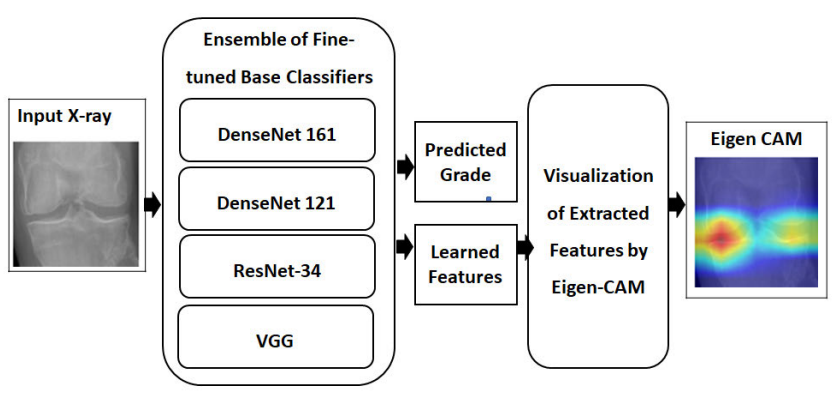
\includegraphics[width=0.8\textwidth]{figs/tariq2023.png}
    \caption{Metodologia proposta por \cite{Tariq2023}.}
    \label{fig:tariq2023}
\end{figure}

No mesmo ano, \cite{domingues2023} propuseram um modelo de RNC baseado na arquitetura DenseNet-161, treinado com um conjunto de radiografias obtidas do Estudo Longitudinal de Saúde do Adulto Musculoesquelético (ELSA-Brasil Musculoesquelético), para a classificação binária automática da OA de joelhos (\autoref{fig:domingues2023}). Eles aplicaram diversas técnicas de pré-processamento, como rotação, desfoque gaussiano e inversão horizontal, e alcançaram uma AUC de 0,866 (IC 95\%: 0,842-0,882), considerando uma média entre os subconjuntos de treino e teste. O modelo também pode ser calibrado por meio do ajuste de limiares (\textit{threshold-moving}, do inglês) para alcançar uma acurácia máxima de 90,7\% e uma sensibilidade de 93,8\%.

\begin{figure}[ht]
    \centering
    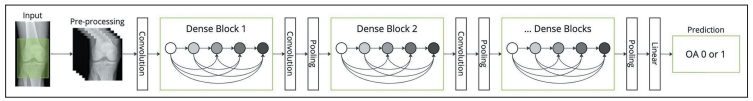
\includegraphics[width=\textwidth]{figs/domingues2023.png}
    \caption{Metodologia proposta por \cite{domingues2023}.}
    \label{fig:domingues2023}
\end{figure}

\cite{Cueva2022} desenvolveram um sistema de diagnóstico por computação assistida (CAD) utilizando a técnica de ajuste fino do modelo ResNet-34 para detectar OA nos dois joelhos simultaneamente (\autoref{fig:cueva2022}). Os autores resolveram o problema de desequilíbrio do conjunto de dados por meio de técnicas de \textit{oversampling} e \textit{data augmentation}, como rotação aleatória e variação de cor. O modelo alcançou uma acurácia média de 61,71\% em múltiplas classes, com melhor desempenho para as classes KL-0, KL-3 e KL-4 em comparação com KL-1 e KL-2 devido às sutis diferenças nos estágios intermediários.

\begin{figure}[ht]
    \centering
    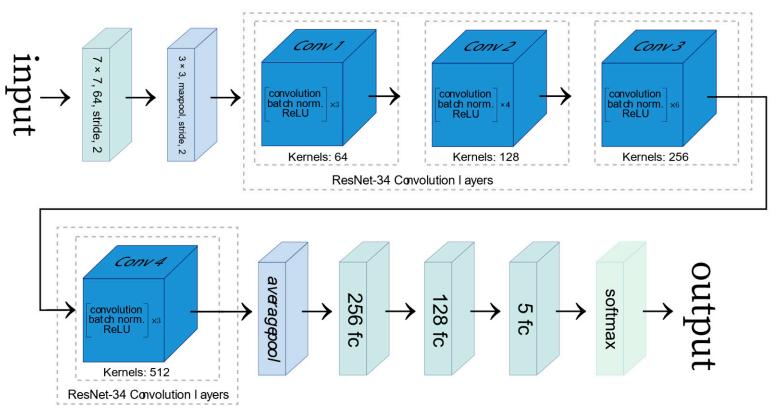
\includegraphics[width=\textwidth]{figs/cueva2022.png}
    \caption{Metodologia proposta por \cite{Cueva2022}.}
    \label{fig:cueva2022}
\end{figure}

Utilizando uma outra abordagem, \cite{yeoh2023} investigaram o uso de redes neurais convolucionais 3D para detecção binária de osteoartrite de joelhos a partir de imagens de ressonância magnética 3D. O estudo também utilizando transferência de aprendizado, transformando pesos de modelos pré-treinados em 2D para 3D. A abordagem permitiu capturar informações espaciais nas três dimensões, resultando em uma acurácia de 87,5\% e um F1-score de 0,871 para o melhor modelo, o ResNet-34.

Com a introdução dos Vision Transformers (ViTs), novas possibilidades surgiram para trabalhar o mesmo problema, oferecendo uma alternativa às RNCs, por vezes superando-as em tarefas de classificação de imagens. Em 2023, \cite{sekhri2023} introduziram uma abordagem utilizando o Swin Transformer para previsão da severidade da OA de joelhos. Para lidar com a alta similaridade entre os graus adjacentes da escala KL, implementaram uma arquitetura de múltiplas previsões composta por cinco redes MLP (Perceptron Multicamadas), cada uma dedicada a prever um grau específico de KL. Além disso, para reduzir o desvio de dados entre os conjuntos de dados (OAI e MOST), congelaram as camadas MLP após o treinamento inicial em um conjunto de dados e continuaram treinando o extrator de características em outro para alinhar os espaços representacionais latentes. Essa abordagem alcançou acurácia de 70,17\% e F1-score de 0,67 no conjunto de dados OAI, superando os métodos existentes do estado da arte.

\begin{figure}[ht]
    \centering
    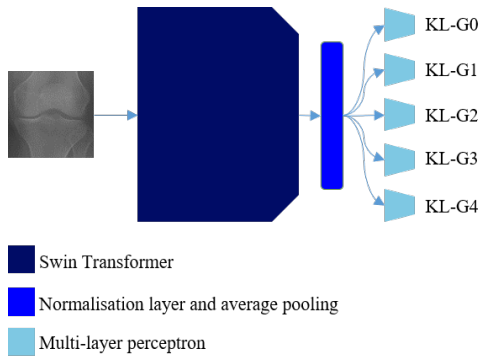
\includegraphics[width=0.7\textwidth]{figs/sekhri2023.png}
    \caption{Metodologia proposta por \cite{sekhri2023}.}
    \label{fig:sekhri2023}
\end{figure}

\cite{Wang_2024} criaram um modelo baseado em ViT para detecção precoce da OA de joelhos, focando na distinção entre o grau KL-0 e KL-2 (\autoref{fig:wang2024}). A metodologia incorporou três inovações principais:

\begin{itemize}
    \item Selective Shuffled Position Embedding (SSPE): Ao fixar o posicionamento de "patches-chave" (regiões com características de grau KL) e embaralhar os demais, o modelo foi forçado a focar nas áreas críticas afetadas pela OA.
    \item Estratégia de troca de patches-chave: Como técnica de aumento de dados, patches-chave de imagens candidatas foram trocados com a imagem alvo para gerar sequências de entrada diversas.
    \item Função de perda híbrida: Uma combinação de Label Smoothing Cross-Entropy (LSCE) para sequências mistas de grau KL e Cross-Entropy (CE) para sequências completas de grau KL foi otimizada para melhorar a generalização do modelo.
\end{itemize}

Essas estratégias resultaram em uma melhoria notável no desempenho de classificação, com o modelo alcançando uma acurácia de 89,80\%.

\begin{figure}[ht]
    \centering
    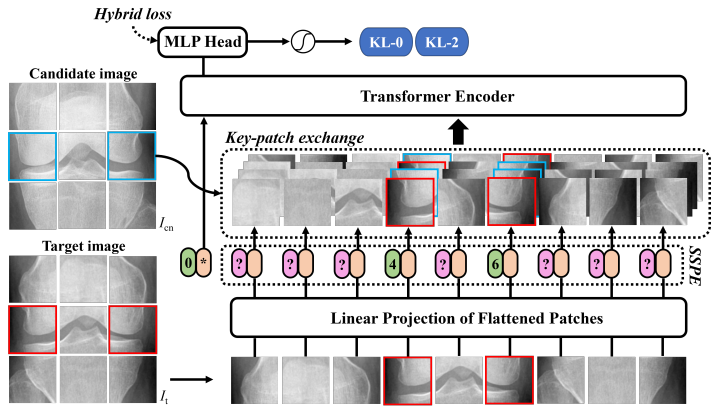
\includegraphics[width=\textwidth]{figs/wang2024.png}
    \caption{Metodologia proposta por \cite{Wang_2024}.}
    \label{fig:wang2024}
\end{figure}

Seguindo uma linha semelhante a este estudo, \cite{apon2024} conduziram uma análise comparativa entre modelos ViT pré-existentes (DaVIT, GC ViT, MaxViT) e RNCs tradicionais (\autoref{fig:apon2024}). Eles destacaram as forças arquitetônicas do DaVIT com autoatenção dupla, do GC ViT com autoatenção de contexto global e do MaxViT com atenção multi-eixo. Esses modelos ViT se destacaram com as melhores métricas, alcançando uma acurácia máxima de 66,14\%, precisão de 0,703, revocação de 0,614 e AUC superior a 0,835, superando consistentemente as RNCs (com acurácia entre 55-65\%).

\begin{figure}[ht]
    \centering
    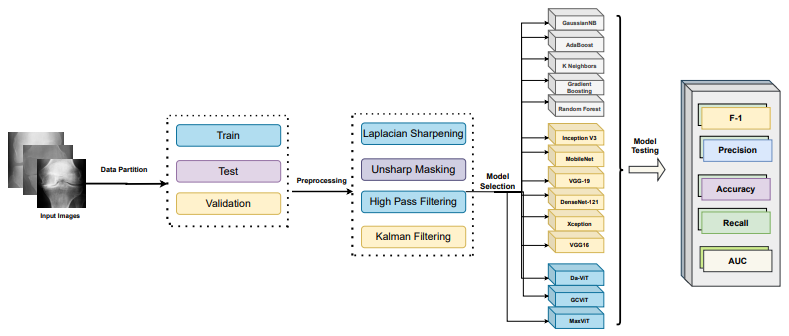
\includegraphics[width=\textwidth]{figs/apon2024.png}
    \caption{Metodologia proposta por \cite{apon2024}.}
    \label{fig:apon2024}
\end{figure}